% !TEX root = ../main.tex
\subsection{Constraints on Galaxy Pitch angle}
\label{section:constraints-on-galaxy-phi}
Our hierarchical model identifies the pitch angle of individual arms ($\phi_\mathrm{arm}$) with posterior standard deviations less than {1.6\degree} for 95\% of arms, assuming no error on disc inclination and position angle. This is illustrated well by the small uncertainties on fit spiral arms in Figure \ref{fig:example-spiral-fits}. The pitch angle of a galaxy as a whole ($\phi_\mathrm{gal}$), however, is not well constrained. This is primarily a result of only having pitch angles measurements for a small number of arms per galaxy, and reflects the difficulty in providing a single value for the pitch angle of a galaxy containing individual arms with very different pitch angles. For galaxies with two arms identified in \textit{Galaxy Builder}, we have a mean uncertainty of ($\sigma_{\phi_\mathrm{gal}}$) of  {7.9\degree}, which decreases to {6.8\degree} and {6.0\degree} for galaxies with three and four arms respectively. This is roughly consistent with the standard error on the mean for a galaxy with $N$ arms,

\begin{figure*}
  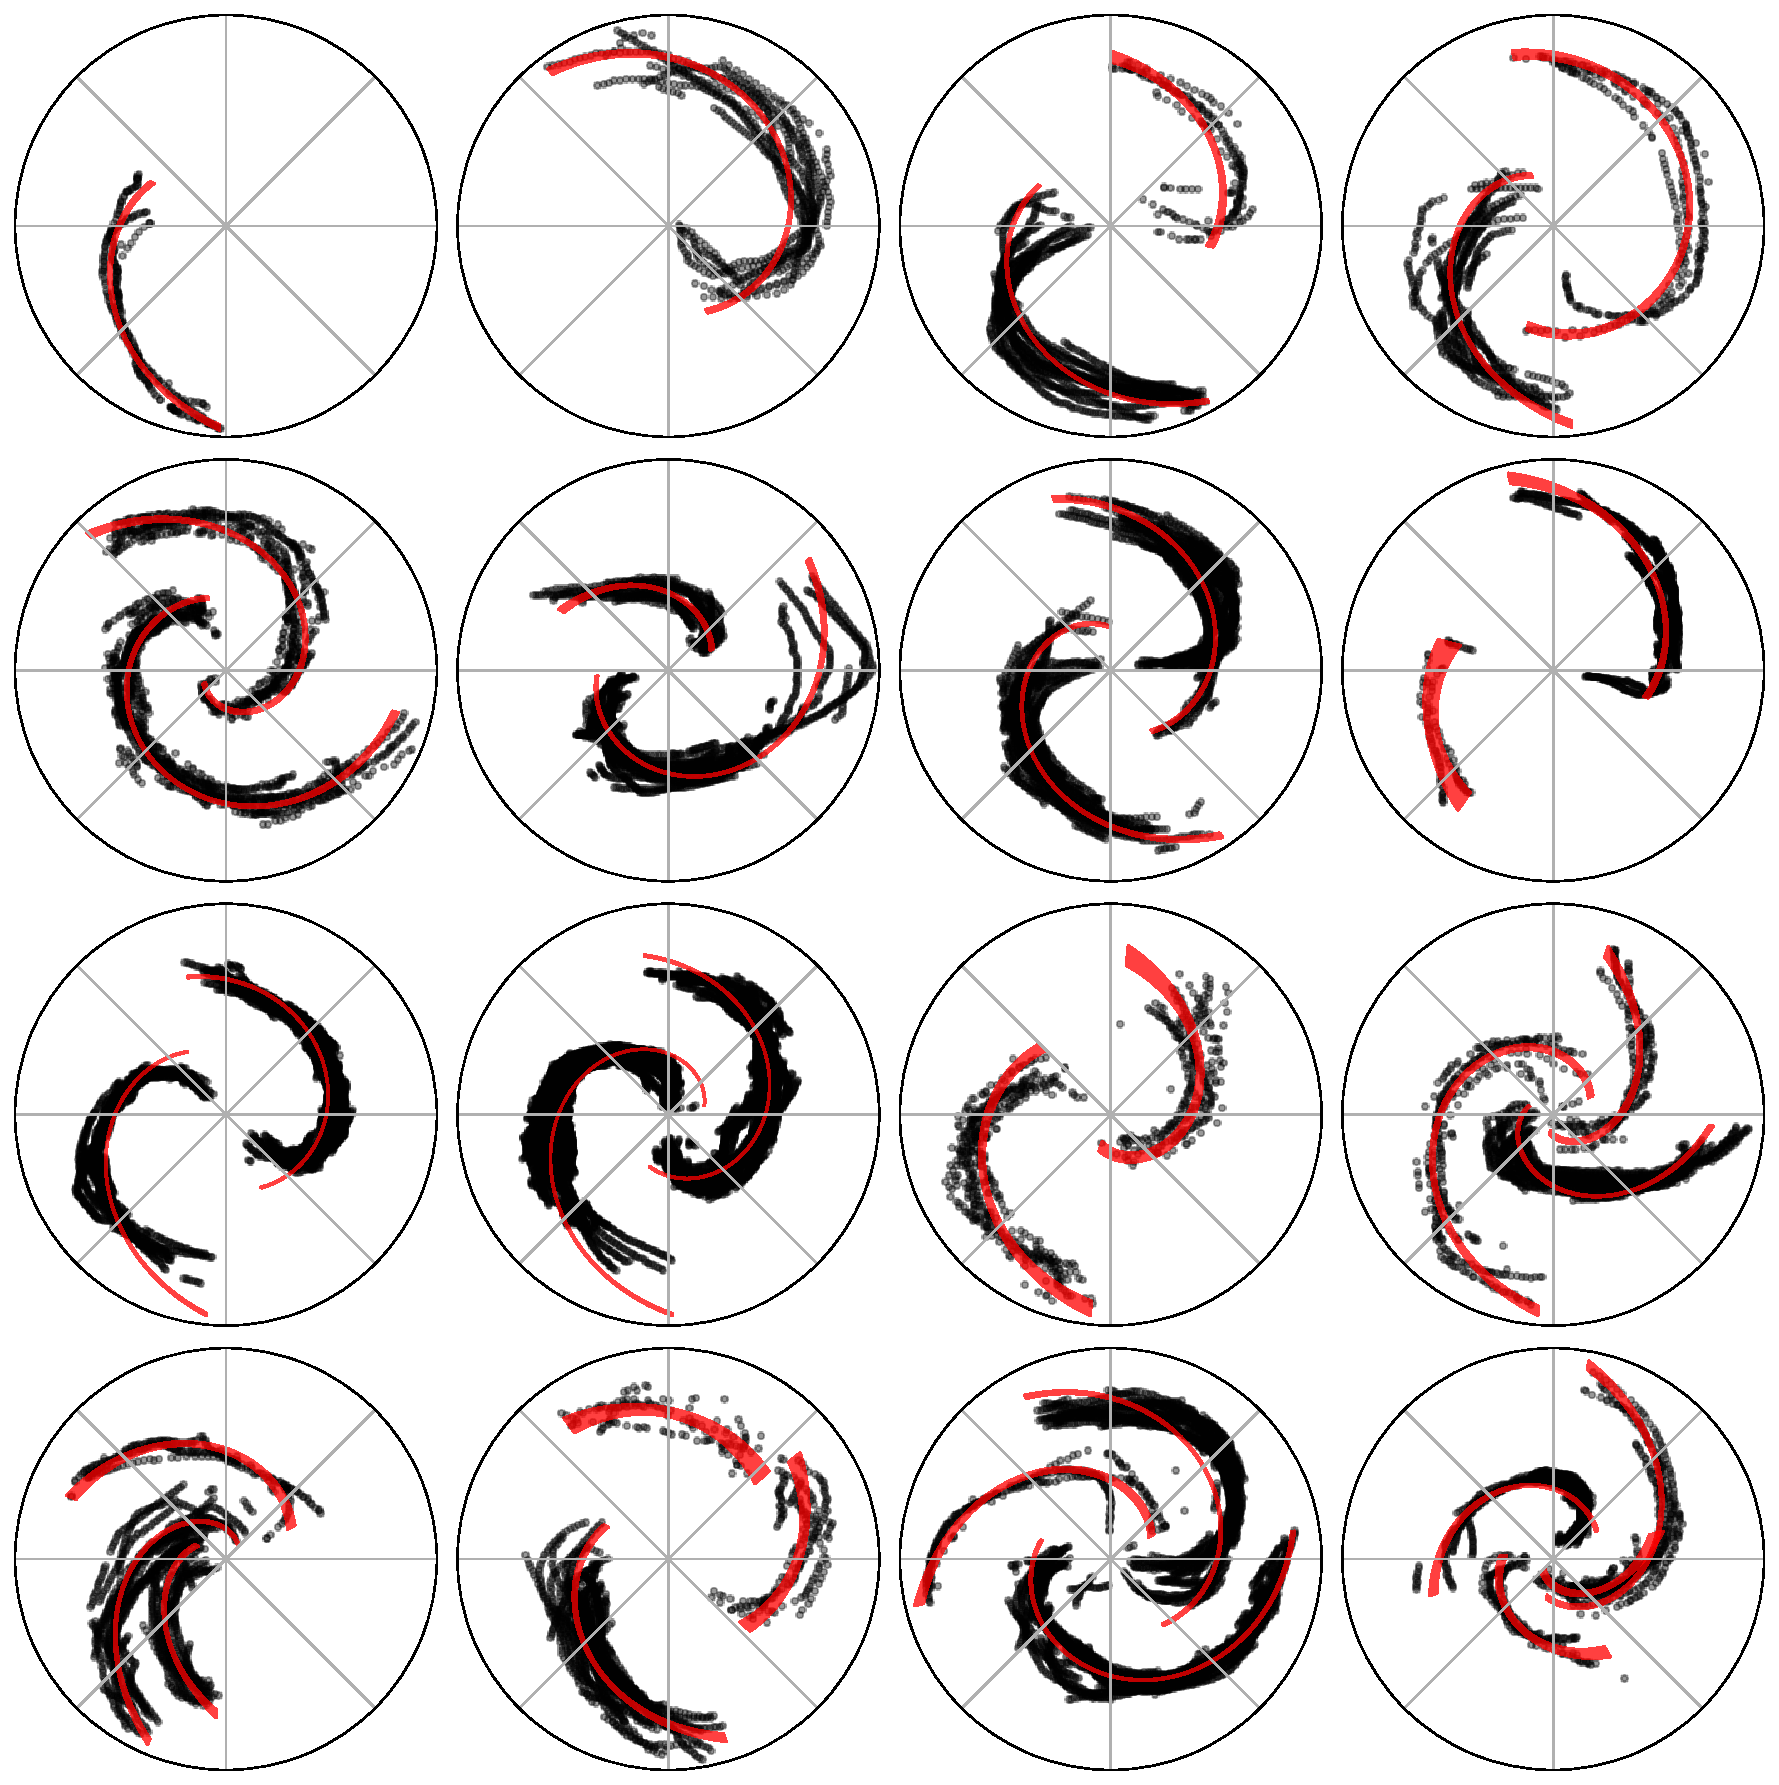
\includegraphics[width=17.7cm]{plots/example-spiral-fits.pdf}
  \caption{Examples of spiral profiles fit using the hierarchical model described in Section \ref{section:bhsm-model}. Deprojected points from \textit{Galaxy Builder} clustered, cleaned spiral arms are shown in black; fit logarithmic spiral arms are shown in red, with the width of the line corresponding to the $2\sigma$ interval on predicted values of $\widetilde{r_\mathrm{arm}}$. The two one-armed spirals in the top left panels are instances where the spiral clustering algorithm failed to identify all spiral arms present in the galaxy.}
  \label{fig:example-spiral-fits}
\end{figure*}

\begin{equation}
  \sigma_{\phi_\mathrm{gal}} = \frac{\sigma_\mathrm{gal}}{\sqrt{N}},
\end{equation}
where $\sigma_\mathrm{gal}$ is our measure of inter-arm variability of pitch angle and has a posterior distribution of $11.0^\circ\pm 0.9^\circ$. This inter-arm variability is similar to that found by \citet{1981AJ.....86.1847K} and \citet{2014ApJ...790...87D} and emphasises the need for fitting algorithms to not assume all arms have the same pitch angle. The spread of arm pitch angle from the mean galaxy pitch angle can be seen in Figure \ref{fig:arm-pa-spread}, with points colour-coded by the number of arms measured for a galaxy. We see a slight drop in the expectation values of galaxy pitch angle ($E[\phi_\mathrm{gal}]$) compared to the expectation of arm pitch angles ($E[\phi_\mathrm{arm}]$) at small galaxy pitch angles, {\bf which is caused by a combination of the} truncation of $\phi_\mathrm{gal}$ at {0\degree} {\bf and the large spread (so the mean value differs from the mode as the distribution is highly skewed).}

\begin{figure*}
  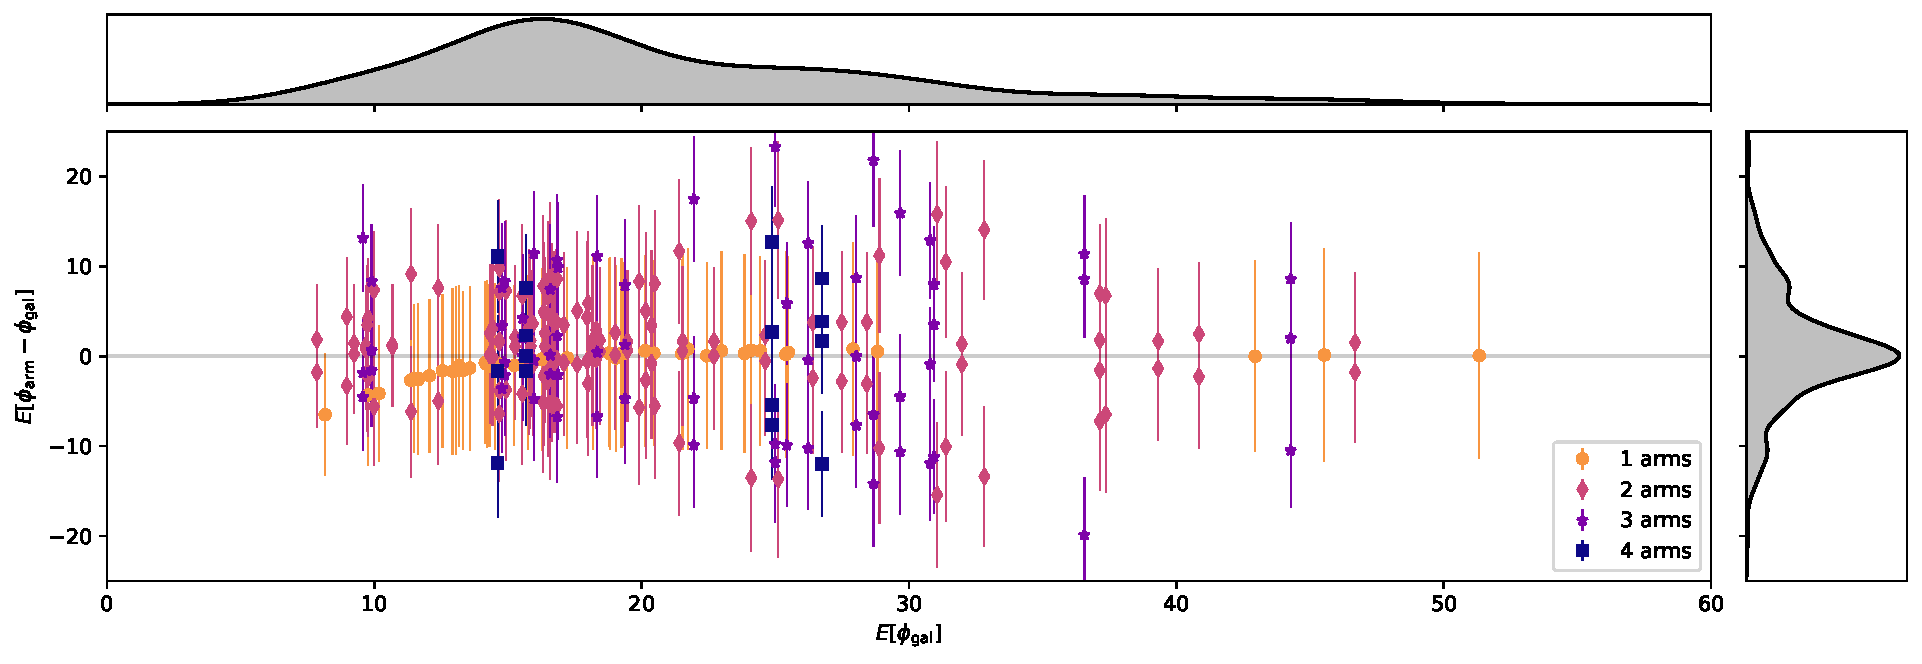
\includegraphics[width=17.7cm]{plots/arm_pa_spread.pdf}
  \caption{Scatter plot showing how arm pitch angle compares to galaxy pitch angle for galaxies with different pitch angles and number of arms. The top panel shows a Gaussian KDE for $E[\phi_\mathrm{gal}]$, and the right panel shows a Gaussian KDE for $E[\phi_\mathrm{arm} - \phi_\mathrm{gal}]$. The galaxy pitch angle is consistent with the mean of its arms, with large scatter and a slight bias against values near the lower bound of $0$ due to the lower limit applied.}
  \label{fig:arm-pa-spread}
\end{figure*}

\textbf{In Figure \ref{fig:stellar-mass-phigal} we present the stellar mass distribution of the sample, and investigate how the global galaxy pitch angle depends on this parameter. The majority of our sample has stellar masses $9.5 < \log(M_* / M_\odot) < 10.0$, and galaxy average pitch angles 10$^\circ$--20$^\circ$. This should be remembered in our physical interpretation of other results. We observe no significant trend of the global pitch angle with mass, although there is a hint that more massive spirals may on average have more tightly wound arms. }

\begin{figure}
  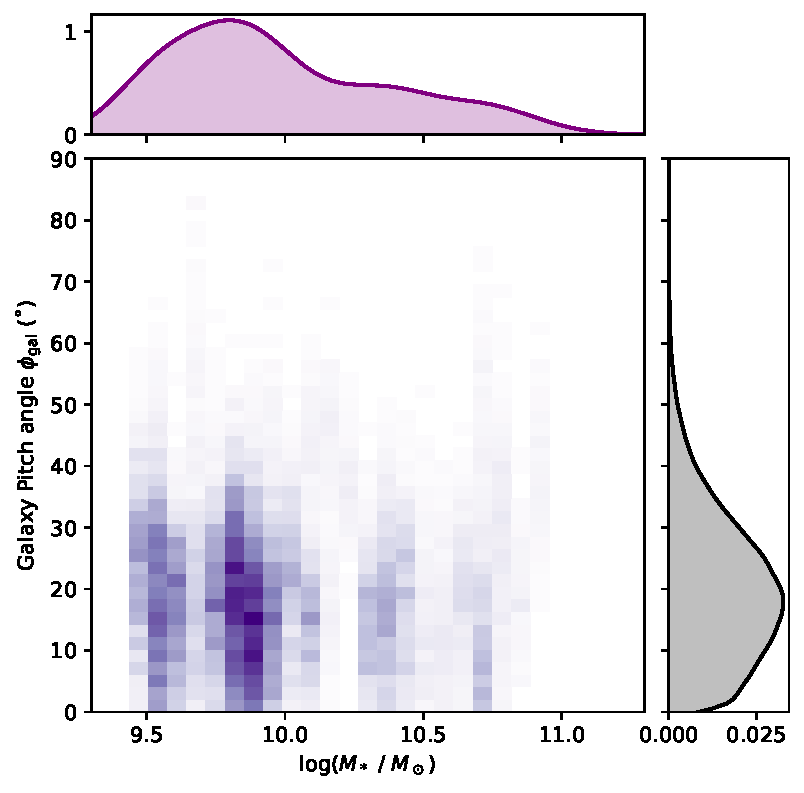
\includegraphics[width=9cm]{plots/stellar_mass_phigal_distribution.pdf}
  \caption{The stellar mass distribution of the sample and the galaxy average pitch angle distribution shown as a 2D histogram (centre) and also projected along each axis. }
  \label{fig:stellar-mass-phigal}
\end{figure}

% for one-armed galaxies = {9.86\degree}

\subsection{Dependence of pitch angle on Galaxy Morphology}
\label{section:morphology-comparison}

To test the possible progenitor distribution of our estimated arm pitch angles, we repeatedly perform an Anderson-Darling test (\citealt{10.2307/2286009}, implemented in \textsc{Scipy}, \citealt{scipy-paper}) over each draw present in the MC trace, resulting in a distribution of Anderson-Darling statistics. We will refer to this test as the \textit{marginalized Anderson-Darling test}. We also make use of the two-sample Anderson-Darling \citep{doi:10.1080/01621459.1987.10478517} test in a similar manner.

We make use of Galaxy Zoo 2 data for morhpological comparison. Two of the galaxies in our sample could not be matched to Galaxy Zoo 2 data, and as such have been dropped from this comparison (leaving 127 galaxies).

\subsubsection{Pitch angle vs. Bulge size}
\label{section:morphology-comparison-bulge}

Morphological classification commonly links bulge size to spiral tightness, and such a link is implied by the Hubble Sequence (\citealt{2005ARA&A..43..581S}, \citealt{2009MNRAS.393.1531G}, \citealt{2013seg..book..155B}), \textbf{although small bulge Sa galaxies have been noted for decades (e.g. for a review see \citet{2005ARA&A..43..581S}; this is also noted in \citealt{2019MNRAS.487.1808M})}. Some recent studies have indeed reported a link between measured spiral galaxy pitch angle and bulge size (i.e. \citealt{2019ApJ...873...85D}), while others have not found any significant correlation \citep{2019MNRAS.487.1808M}. \textbf{The differing results of this may depend on the details of how both the bulge size, and spiral pitch angles are measured and suggest further investigation is needed.} We investigate this relationship here using a measure of bulge prominence from Galaxy Zoo 2, as Equation 3 in \citet{2019MNRAS.487.1808M}:

\begin{equation}
  B_\mathrm{avg} = 0.2\times p_\mathrm{just\ noticeable} + 0.8\times p_\mathrm{obvious} + 1.0\times p_\mathrm{dominant},
\end{equation}
where $p_\mathrm{just\ noticeable}$, $p_\mathrm{obvious}$ and $p_\mathrm{dominant}$ are the fractions of classifications indicating the galaxy's bulge was ``just noticeable'', ``obvious'' or ``dominant'' respectively.

We see no correlation between galaxy pitch angle derived from the hierarchical model and $B_\mathrm{avg}$. The Pearson correlation coefficient between the expectation value of galaxy pitch angle ($E[\phi_\mathrm{gal}]$) and $B_\mathrm{avg}$ is 0.00 (with a p-value of 0.95).

\begin{figure*}
  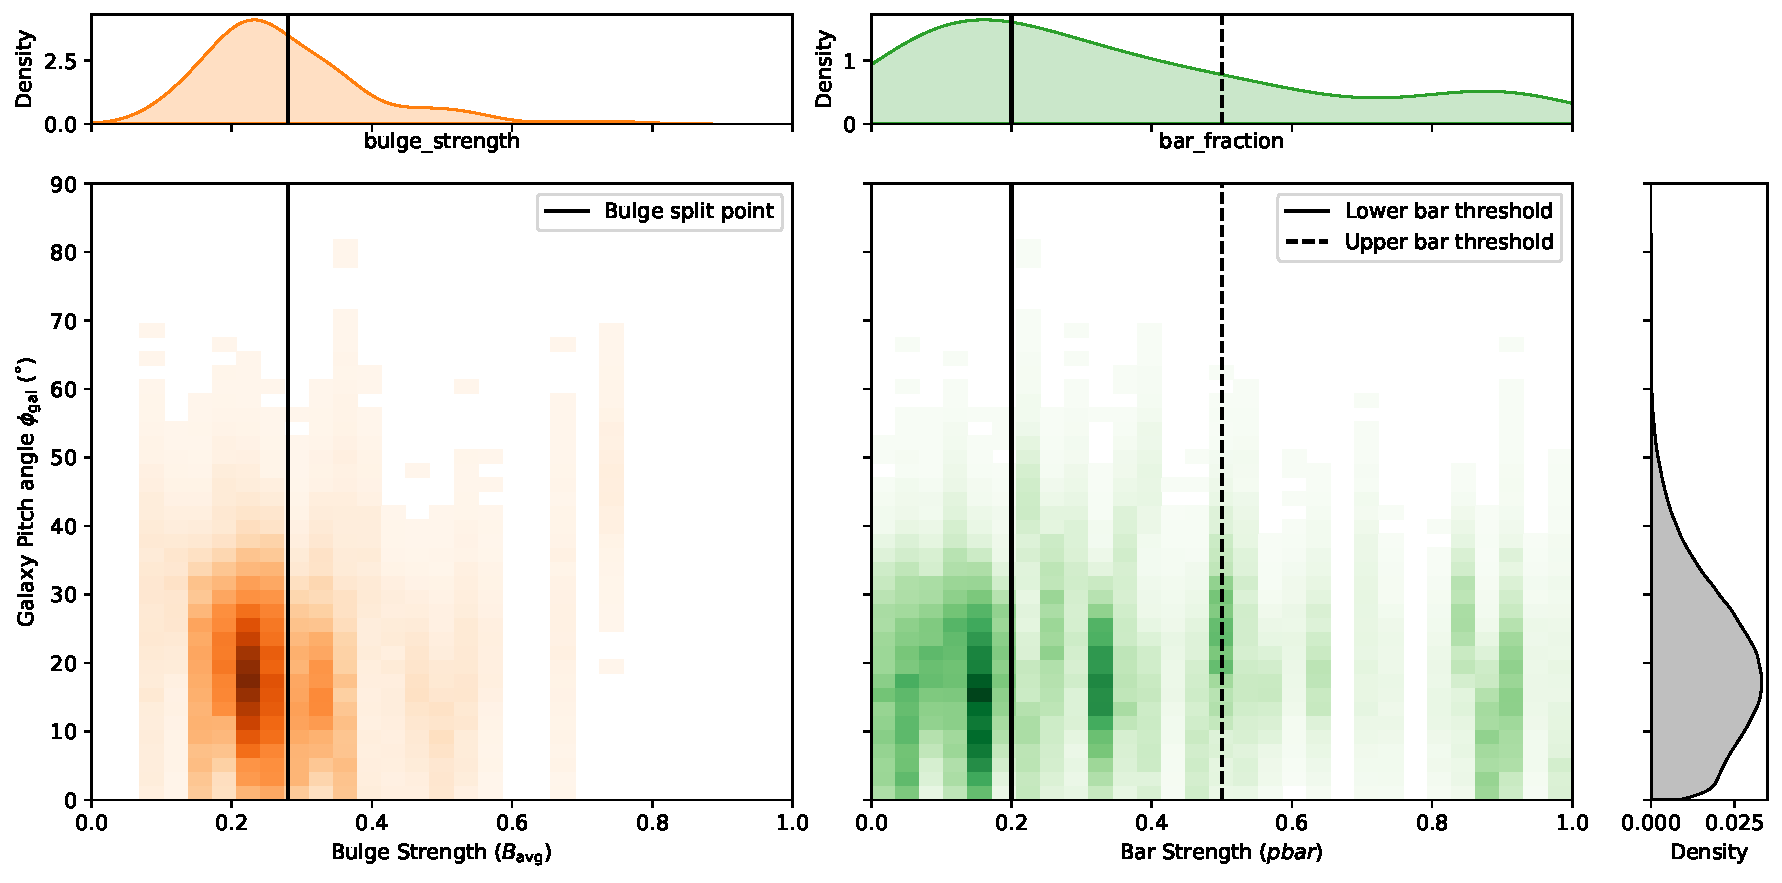
\includegraphics[width=17.7cm]{plots/bulge_bar_phigal_distribution.pdf}
  \caption{Density plot showing bulge strength ($B_\mathrm{avg}$; left, orange) and bar strength ($p_\mathrm{bar}$; right, green) against galaxy pitch angle ($\phi_\mathrm{gal}$). Split points for the marginalized Anderson-Darling tests are labelled. There is no statistically significant relationship for either bulge or bar strength.}
  \label{fig:bulge-bar-pa-hist}
\end{figure*}

We separate our sample into galaxies with weaker bulges ($B_\mathrm{avg} < 0.28$, 79 galaxies) and those with stronger bulges ($B_\mathrm{avg} \ge 0.28$, 48 galaxies), to test whether their pitch angles could be drawn from significantly different distributions. A marginalized two-sample Anderson-Darling test comparing the distributions of $\phi_\mathrm{gal}$ for the samples does not find evidence that galaxy pitch angles were drawn from different distributions: we reject the null hypothesis at the 1\% level for only 1\% of the samples. Similarly comparing arm pitch angles for galaxies in the different samples results in not rejecting the null hypothesis at the 1\% level for any of the samples. The distributions of the Anderson-Darling test statistic for $\phi_\mathrm{gal}$ and $\phi_\mathrm{arm}$ are shown in the upper panel of Figure \ref{fig:ad-morphology-test} in blue and orange respectively.

One limitation of this result is that our sample does not contain many galaxies with dominant bulges: $B_\mathrm{avg}$ only varied from 0.09 to 0.75 (the allowed maximum being 1.0), with only four galaxies having $B_\mathrm{avg} > 0.5$. The split point of 0.28 was also chosen to produce evenly sized comparison samples rather than from some physical motivation. However, the lack of any form of correlation implies that there is no evidence in our data for the link between bulge size and pitch angle predicted by the Hubble sequence and observed in other studies.

\subsubsection{Pitch angle vs. Bar Strength}
\label{section:morphology-comparison-bar}

One of the predictions of Manifold theory is that pitch angle increases with bar strength \citep{2009MNRAS.400.1706A}. \textbf{In this work we do not have any direct measurement of bar strength; nor are there significant numbers of strongly barred galaxies in our sample. However in an attempt to} investigate this relationship in our data, we make use of Galaxy Zoo 2's bar fraction ($p_\mathrm{bar}$), which has been demonstrated to be a good measure of bar length \citep{Willett2013:1308.3496v2} and bar strength \citep{2012MNRAS.423.1485S,2012MNRAS.424.2180M,2018MNRAS.473.4731K} and therefore a good measure of the torque applied on the disc gas.

We do not observe a correlation between $p_\mathrm{bar}$ and $E[\phi_\mathrm{gal}]$ (Pearson correlation coefficient of -0.05, with a p-value of 0.54). Following \citet{2012MNRAS.424.2180M} and \citet{2012MNRAS.423.1485S}, we separate the sample into galaxies without a bar ($p_\mathrm{bar} < 0.2$, 50 galaxies), with a weak bar ($0.2 \le p_\mathrm{bar} \le 0.5$, 44 galaxies) and with a strong bar ($p_\mathrm{bar} > 0.5$, 33 galaxies). Performing marginalized three-sample Anderson-Darling tests does not find that pitch angles ($\phi_\mathrm{gal}$ or $\phi_\mathrm{arm}$) of galaxies with different bar strengths were drawn from different distributions; we do not reject the null hypothesis at the 1\% level for any samples for the test of $\phi_\mathrm{gal}$, and at the 10\% level for the test of $\phi_\mathrm{arm}$. The distributions of Anderson-Darling test statistic is shown in the lower panel of Figure \ref{fig:ad-morphology-test}.

\begin{figure*}
  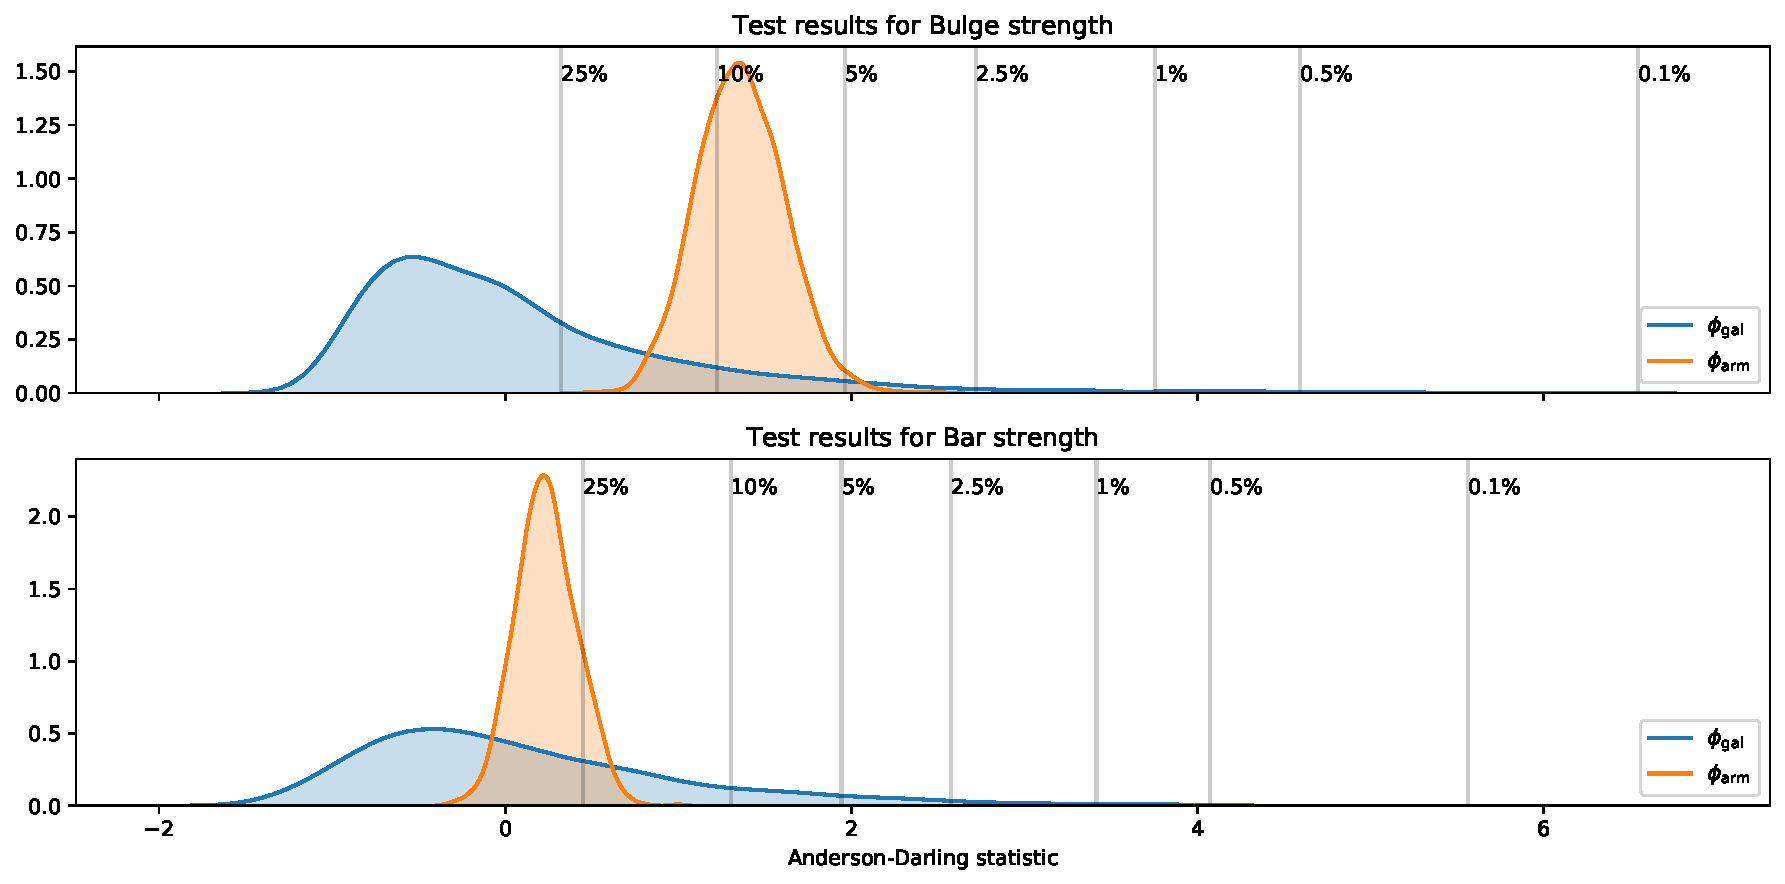
\includegraphics[width=17.7cm]{plots/bulge_bar_test_results.pdf}
  \caption{The results of marginalized two-sample Anderson-Darling tests examining whether pitch angles ($\phi_\mathrm{gal}$ in blue and $\phi_\mathrm{gal}$ in orange) for galaxies with $B_\mathrm{avg} < 0.28$ and $B_\mathrm{avg} \ge 0.28$ are drawn from the same distribution (top panel), and the results of marginalized three-sample Anderson-Darling tests for galaxies with no bar ($p_\mathrm{bar} < 0.2$), a weak bar ($0.2 \le p_\mathrm{bar} \le 0.5$) and a strong bar ($p_\mathrm{bar} > 0.5$) (bottom panel). Confidence intervals are shown, with moving rightwards indicating more confidence in rejecting the null hypothesis that the compared values were drawn from the same parent distribution. We cannot reject the null hypotheis at the 1\% level for any of the tests conducted, meaning there is no evidence in this sample that bulge size or bar strength impacts pitch angle.}
  \label{fig:ad-morphology-test}
\end{figure*}

The fact that we do not find any link between \textbf{our measure of bar strength (based on the prominance of the bar in Galaxy Zoo 2) and pitch angle is suggestive that there is actually no link between bar strength and pitch angle, which would exclude Manifold theory as the primary mechanism driving the evolution of the spirals in our sample. However since we use only a proxy for bar strength, which has not been well tested, this is not conclusive.}

\subsection{Spiral Winding}
\label{section:spiral_winding}

For transient and recurrent spiral arms driven by self-gravity, \citet{2019arXiv190910291P} suggest that spiral patterns form at some maximum pitch angle ($\phi_\mathrm{max}$), continually wind up over time and finally dissipate at some minimum pitch angle ($\phi_\mathrm{min}$). They propose that, under a set of very simple assumptions, the evolution of pitch angle would be governed by

\begin{equation}
  \label{eq:winding}
  \cot{\phi} = \left[R\frac{\mathrm{d}\Omega_p}{\mathrm{d}R}\right](t - t_0) + \cot{\phi_\mathrm{max}},
\end{equation}
where $\Omega_p$ is the radially dependant pattern speed of the spiral arm and $t_0$ is the initial time at which it formed.

In QSDW theory, the pattern speed $\Omega_p$ is a constant in R, as spiral arms obey rigid-body rotation. If $\Omega_p$ instead varies with radius we would expect $\cot{\phi}$ to be uniformly distributed between $\cot{\phi_\mathrm{max}}$ and $\cot{\phi_\mathrm{min}}$. {\bf The model presented in \citet{2019arXiv190910291P} does not give any physical justification for what $\cot{\phi_\mathrm{max}}$ and $\cot{\phi_\mathrm{min}}$ should be. }

To test this theory, \citet{2019arXiv190910291P} used a Kolmogorov-Smirnov test to examine whether {\bf a sample of 113} galaxies with measured pitch angles was likely to have been drawn from a distribution uniform in its cotangent. Pitch angles were measured {\bf by \citet{2019ApJ...871..194Y}} using discrete Fourier transformations in one- and two-dimensions, and as such do not account for inter-arm variations. They {\bf conclude the model works within limits of} $\cot{\phi} \in [1.00, 4.75]$ (roughly $11.9^\circ < \phi < 45.0^\circ$), motivated by examination of the data.

We perform a similar test in this work, using our sample and methods. We will make use of the marginalized Anderson-Darling test described above, and examine winding on a per-arm basis, as well as a per-galaxy basis. Observation of the distribution of arm pitch angles in our sample (Figure \ref{fig:pa-cot-distributions}) suggests {\bf they are close to uniform in cotangent} within limits of $15^\circ < \phi < 50.0^\circ$.

\subsubsection{Galaxy Pitch angle}

Testing the uniformity of $\cot\phi_\mathrm{gal}$ between {15\degree} and {50\degree} using a marginalized Anderson-Darling test results in rejecting the null hypothesis at the 1\% level for just 5\% of samples, with a large spread in observed test values. The full distribution of Anderson-Darling statistics can be seen in Figure \ref{fig:ad-cot-test}. The large spread in results is caused by the large uncertainties in $\phi_\mathrm{gal}$.

This result suggests that \sout{we cannot rule out} {\bf our data are consistent with} a cot-uniform source distribution for galaxy pitch angle, but the large uncertainty in $\phi_\mathrm{gal}$ makes it difficult to make any conclusive statements. This result is also highly sensitive to the lower limit of $\phi$: decreasing it to {10\degree} results in us rejecting the cot-uniform model at greater than the 0.1\% level for 96\% of the posterior samples. {\bf We can conclude from this that the \citet{2019arXiv190910291P} cot-uniform model is an adequate fit to the data, as long as the minimum pitch angle, $\cot{\phi_\mathrm{min}}$, at which the majority of winding dissipate or disappear is  $\phi_\mathrm{min} > $ {10\degree}, and more confidently $\phi_\mathrm{min} = $ {15\degree}. We reiterate that there is no prediction in \citet{2019arXiv190910291P} as to what this minimum pitch angle should be, so our observation constrains the allowed range.} \sout{As we have no information available on the selection biases present for classification of extremely loose or tight spiral arms in \textit{Galaxy Builder}, we choose to keep the less strict limit of {15\degree}.}

\subsubsection{Arm Pitch angle}
The inconclusive result for $\phi_\mathrm{gal}$ is perhaps unsurprising: were we to assume that spiral arms are transient and recurrent instabilities, there is little reason for all of the arms to be at precisely the same evolutionary stage at the same time. This is supported by the large observed spread in inter-arm pitch angles (Section \ref{section:constraints-on-galaxy-phi}).

If we assume instead that spirals form and wind independently inside a galaxy, and that their evolution over time can be described by Equation \ref{eq:winding}, the distribution of the cotangent of pitch angles of individual arms should be uniform between our limits, rather than that of the galaxy's pitch angle as a whole.

Using the marginalized Anderson-Darling test we cannot reject the null hypothesis at even the 5\% level for any of the possible realizations of arm pitch angle. The resulting distribution of Anderson-Darling statistics is shown in in the lower panel of Figure \ref{fig:ad-cot-test}. This result is highly consistent with the model for spiral winding proposed by \citet{2019arXiv190910291P} {\bf with $\cot{\phi_\mathrm{min}} = $ {15\degree} } and can be interpreted as evidence that spirals are formed through local disc perturbations, and are primarily governed by local forces.

\begin{figure*}
  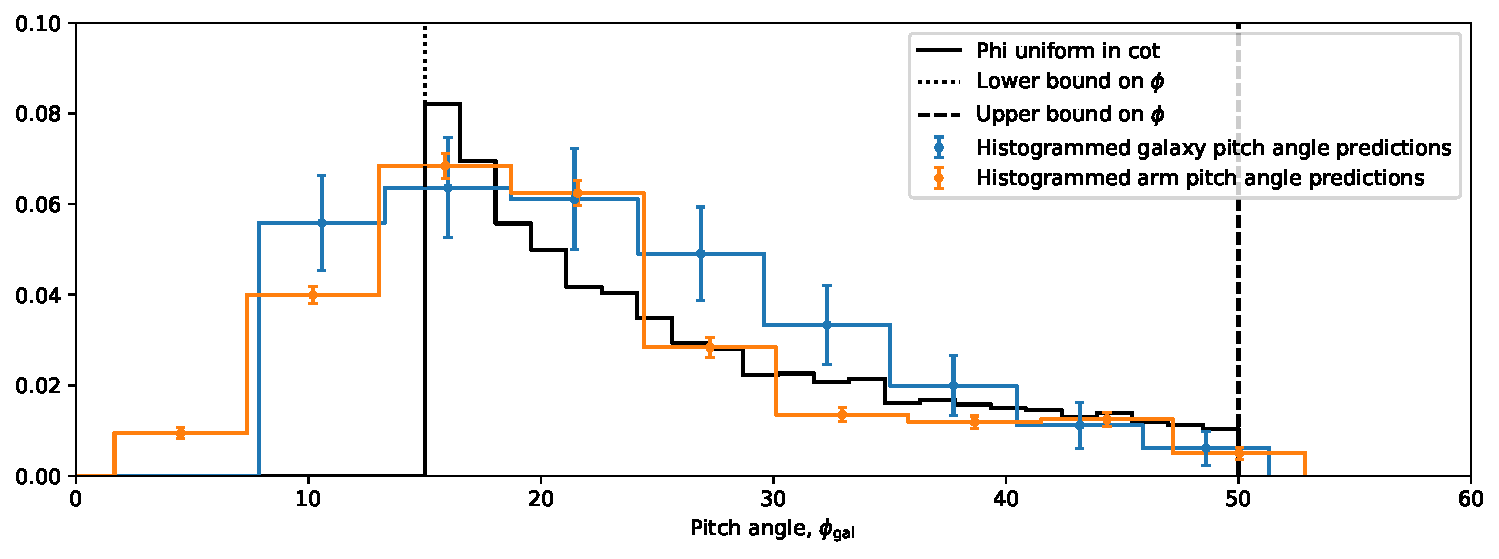
\includegraphics[width=17.7cm]{plots/phi_distribution_comparison.pdf}
  \caption{The distributions of pitch angles (orange and blue) relative to one uniform in $\cot\phi$ (black). Histograms have been normalised by the area between the limits such that they are comparable. The histogram was recalculated with identical bins for each posterior sample of $\phi_\mathrm{gal}$ and $\phi_\mathrm{arm}$, we plot the mean value of each bin, with the sample standard deviation shown as error bars. It is evident that the distributions are very similar between the chosen limits.}
  \label{fig:pa-cot-distributions}
\end{figure*}


\begin{figure*}
  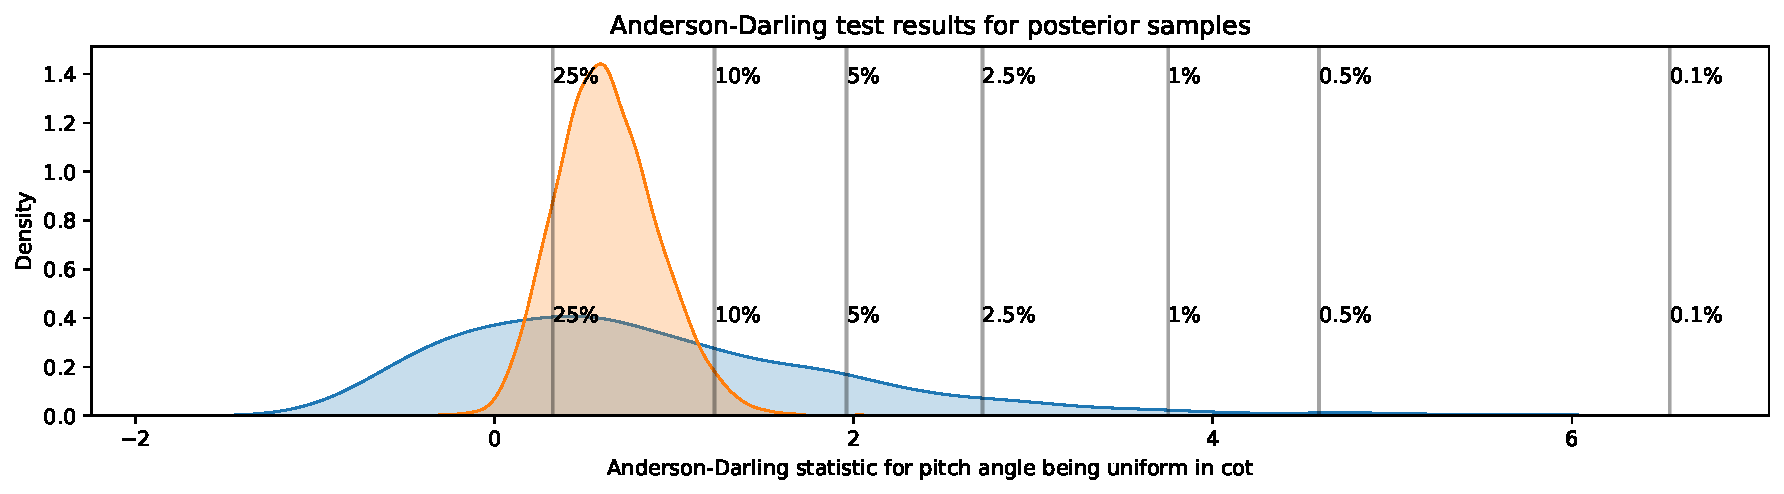
\includegraphics[width=17.7cm]{plots/combined_cot_uniform_marginalized_tests.pdf}
  \caption{The results of a marginalized Anderson-Darling test for uniformity in $\cot$ for $\phi_\mathrm{gal}$ (blue) and $\phi_\mathrm{arm}$ (orange), with values corresponding to various confidence intervals shown. Moving rightwards on the x-axis implies greater confidence in rejecting the null hypothesis that the sample was drawn from a distribution uniform in $\cot$ between $15^\circ < \phi < 50.0^\circ$. In this instance, we would not be able to reject the null hypothesis at the 1\% level for either $\phi_\mathrm{gal}$ or $\phi_\mathrm{arm}$, meaning our sample is consistent with a cot uniform distribution. {\bf The larger error in $\phi_\mathrm{gal}$  means that this result is more significant for $\phi_\mathrm{arm}$, which is also physically motivated, as arms can wind independently.}}
  \label{fig:ad-cot-test}
\end{figure*}
